
\begin{frame}[ctb!]
  \frametitle{Resource Exchange Generality}

  To determine a supply-demand resource exchange for \textit{general} facilities
  in the fuel cycle, information about both the supply and demand must be known.

  \vspace{0.2cm}
  
  For example:
  \begin{itemize}
    \item enrichment facilities - production constraints
    \item reactors - fuel requests
    \item fabrication facilities - fuel supply
  \end{itemize}
  
\end{frame}

\begin{frame}[ctb!]
  \frametitle{Resource Exchange Generality}

  \begin{figure}
    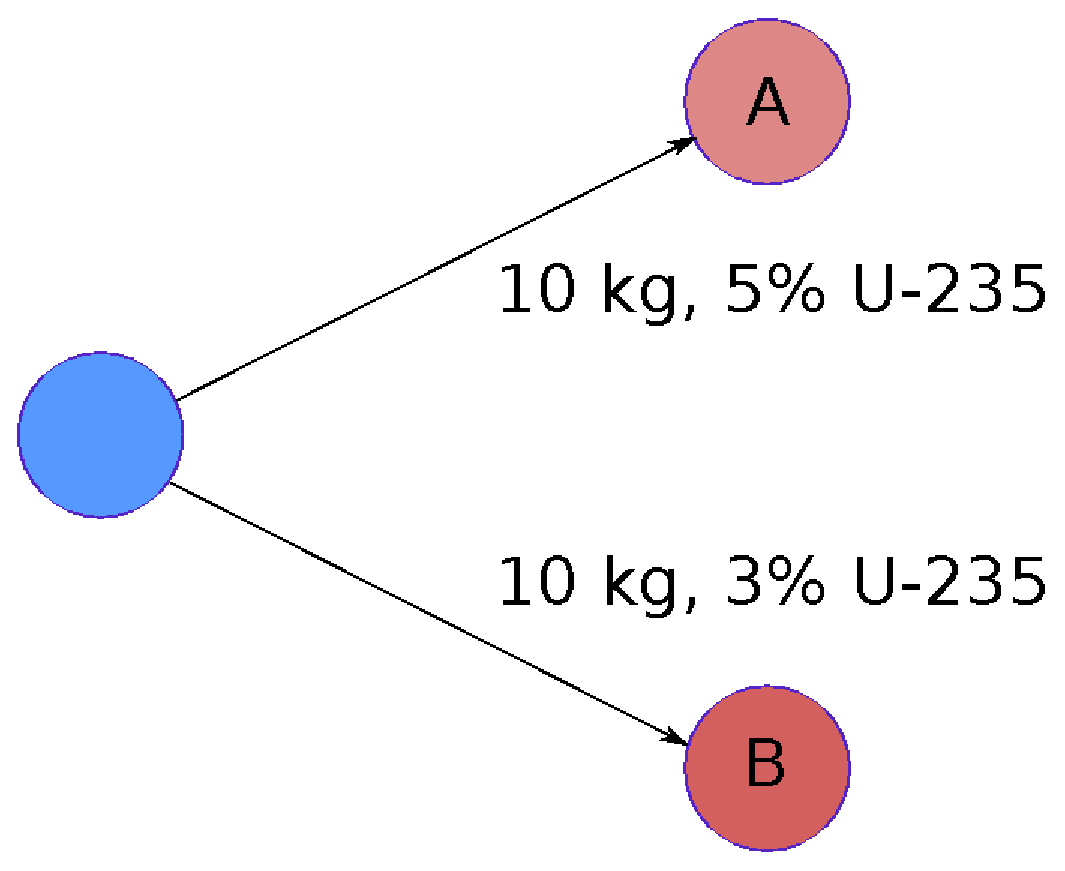
\includegraphics[height=3cm]{./images/enr.eps}
    \caption{Two Demands for Enriched Uranium}
  \end{figure}
  
  \begin{table} [h!]
    \begin{tabular}{|c|c|c|}
      \hline  
      Order & SWU & Nat'l U (kg) \\
      \hline  
      A & 71 & 112\\
      B & 34 & 64\\
      \hline  
    \end{tabular}
  \end{table}

\end{frame}

\begin{frame}[ctb!]
  \frametitle{Resource Exchange Generality}

  This proposal generalizes the exchange of resources in two steps:

  \begin{enumerate}
    \item Gather the information required to make a material flow decision
    \item Solve for material flow
  \end{enumerate}
\end{frame}

\begin{frame}[ctb!]
  \frametitle{Resource Exchange Information Gathering}

  Inspiration taken from Julka et. al. \cite{julka_agent-based_2002},

  \begin{itemize}
    \item fuel cycle is a supply chain
    \item individual facilities are agents
    \item petroleum industry also deals with material quality
  \end{itemize}
  
\end{frame}

\begin{frame}[ctb!]
  \frametitle{Resource Exchange: Request for Bids}
  \begin{figure}
    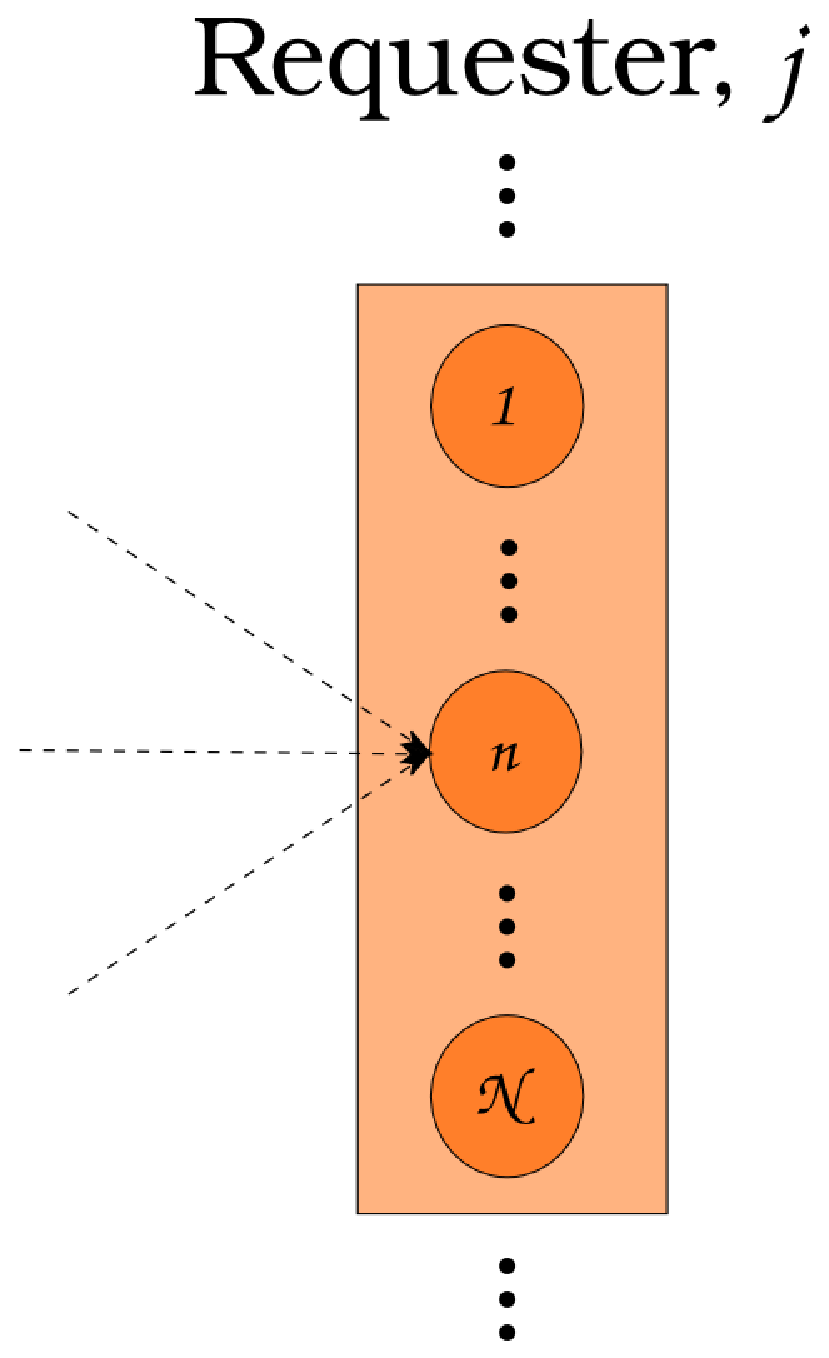
\includegraphics[height=5cm]{./images/requester.eps}
    \caption{Consumers define their demand for commodities during the Request
      for Bids (RFB) phase.}
  \end{figure}
\end{frame}

\begin{frame}[ctb!]
  \frametitle{Resource Exchange: Response to Request for Bids}
  \begin{figure}
    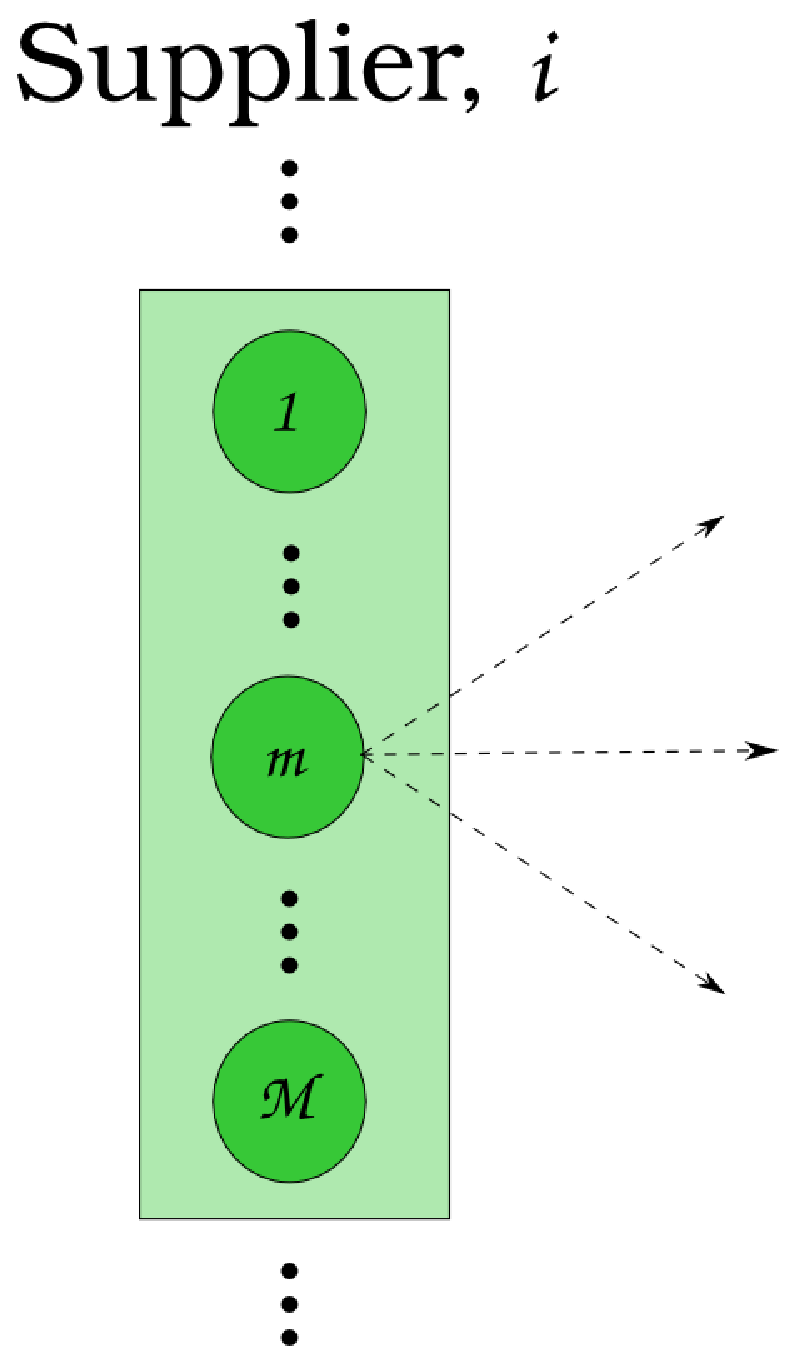
\includegraphics[height=5cm]{./images/supplier.eps}
    \caption{Suppliers respond to each request during the Response to Request
      for Bids (RRFB) phase.}
  \end{figure}
\end{frame}

\begin{frame}[ctb!]
  \frametitle{Resource Exchange: Preference Adjustment}
  \begin{figure}
    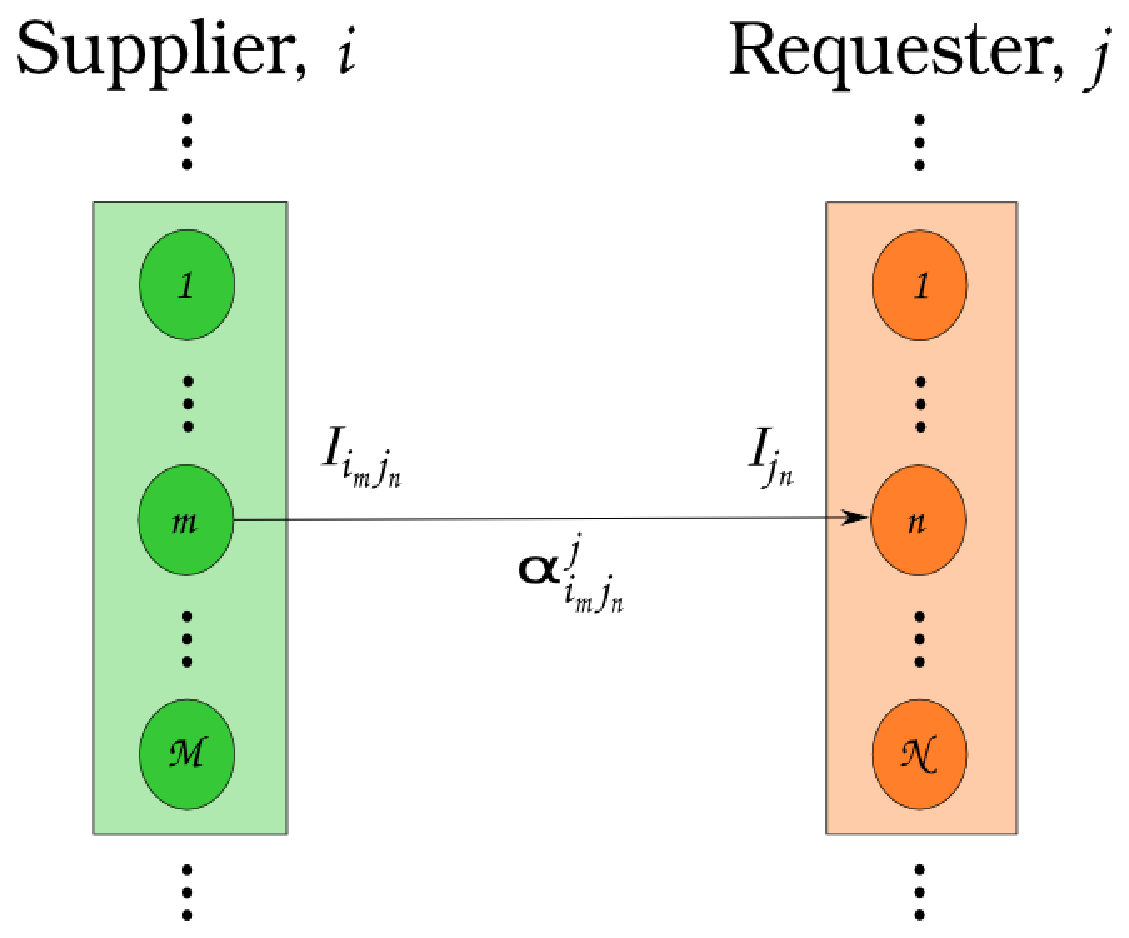
\includegraphics[height=4cm]{./images/supplier-requester.eps}
    \caption{Consumers adjust preferences based on Supplier-given information
      during the Preference Adjustment (PA) phase.}
  \end{figure}

  Managers of facilities (institutions, regions) are then allowed to perturb
  preferences.
\end{frame}

\begin{frame}[ctb!]
  \frametitle{Resource Exchange: Full Picture}
  \begin{figure}
    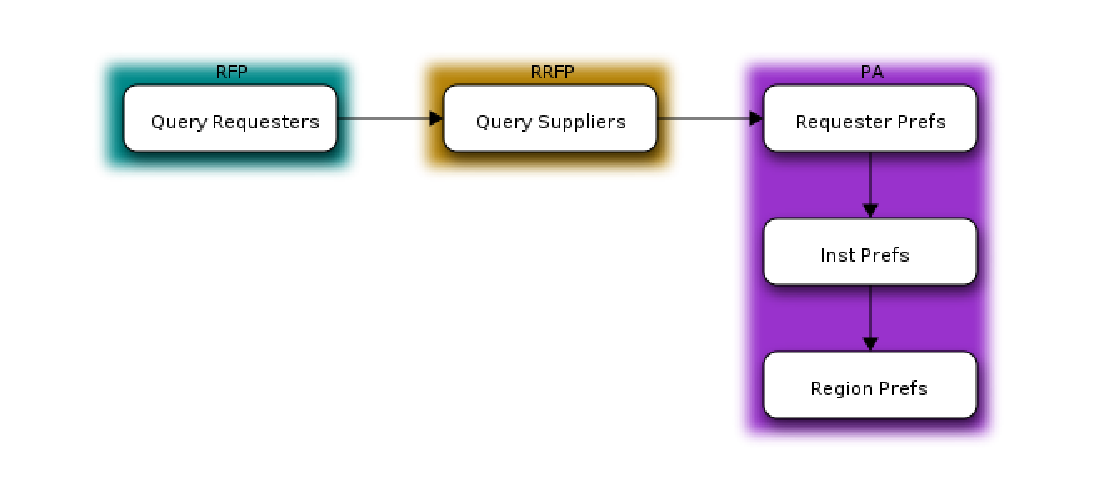
\includegraphics[height=5cm]{./images/exchange.eps}
    \caption{A flow chart of the information gathering phases.}
  \end{figure}
\end{frame}

\begin{frame}[ctb!]
  \frametitle{Resource Exchange Solution Mechanism}

  A Multicommodity Transportation Problem (MTP) formulation naturally fits the
  requirements of the simulation.

  \begin{itemize}
    \item supplier and consumer facilities
    \item discrete transfers of commodities
    \item demand can be met by multiple commodities
  \end{itemize}

  Departs from classic MTP, thus is called Generic Fuel Cycle Transportation
  Problem (GFCTP).
  
\end{frame}

\begin{frame}[ctb!]
  \frametitle{GFCTP - Overview}
  
  The Generic Fuel Cycle Transportation problem assumes the following:
  \begin{itemize}
    \item there is a set of suppliers, a set of requesters, a set of
      commodities, and a set of possible resource transfers, defining arcs
      between suppliers and requesters
    \item a cardinal preference ordering is defined over the set of possible
      resource transfers
    \item suppliers can be constrained both by resource quantities and qualities
    \item multiple commodity types may satisfy a consumer
  \end{itemize}

  A linear programming (LP) formulation and mixed integer-linear programming
  (MILP) formulation is proposed.

\end{frame}
  

\begin{frame}[ctb!]
  \frametitle{GFCTP - Nomenclature}

  Nomenclature used:
  \begin{itemize}
    \item set of commodities, $H$
    \item set of suppliers, $I$
    \item set of requesters, $J$
    \item flow, $x^h_{i,j}$
  \end{itemize}

\end{frame}

\begin{frame}[ctb!]
  \frametitle{GFCTP (LP) - Request Constraint}
  
  Requests
  \begin{itemize}
    \item can be met by multiple commodities, e.g., UOX and MOX
    \item are comprised of
      \begin{itemize}
        \item a quantity, $d_j$
        \item a set of commodities, $H_j$
      \end{itemize}
  \end{itemize}

  \begin{equation}
    \sum_{i \in I}\sum_{h \in H_{j}} x_{i,j}^{h} \geq d_{j}(H_{j})  \: \forall j \in J
  \end{equation}
  
  Feasibility can be guaranteed by using ``fake'' supplier with negative
  preference or infinite cost.

\end{frame}

\begin{frame}[ctb!]
  \frametitle{GFCTP (LP) - Supply Constraint - Example}

  Supply
  \begin{itemize}
    \item can have multiple possible constraints
    \item constraints can be functions of quality and quantity
  \end{itemize}

  E.g., an enrichment facility that provides the commodity enriched uranium (ER):
  \begin{itemize}
    \item A processing constraint, which has units of SWU
    \item An inventory constraint, which has units of kilograms of natural
      uranium (NU)
  \end{itemize}

\end{frame}

\begin{frame}[ctb!]
  \frametitle{GFCTP (LP) - Supply Constraint - Example}
  
  Given
  \begin{itemize}
    \item a requested enrichment level, $\varepsilon_j$
    \item a supply capacity, $s$
    \item a conversion function, $f$
  \end{itemize}

  Associated constraints are
  \begin{equation}
    \sum_{j \in J} f_{SWU}(\varepsilon_j) x_{i,j}^{EU} \leq s_{i,SWU} 
  \end{equation}

  \begin{equation}
    \sum_{j \in J} f_{NU}(\varepsilon_j) x_{i,j}^{EU} \leq s_{i,NU} 
  \end{equation}

  \pause

  These constraints are a function of the isotopic profile of the request, or
  \textit{quality}, $q_j$. More generally suppliers may have conversion
  functions, which are functions of the request quality,
  $\beta_{i,k}(q_{j}^{h})$.

\end{frame}

\begin{frame}[ctb!]
  \frametitle{GFCTP (LP) - Supply Constraint}

  Associated constraints are
  \begin{equation}
    \sum_{j \in J}\beta_{i,k}(q_{j}^{h}) x_{i,j}^{h} \leq s_{i,k} 
    \: \forall \: k \in K_{i}^{h},  
    \forall \: i \in I, \forall \: h \in H
  \end{equation}

  with notation defined as
  \begin{itemize}
    \item $h$ - a commodity
    \item $K_i^h$ - a set of constraints
    \item $s_{i,k}$ - a supply capacity
    \item $\beta_{i,k}(q_{j}^{h})$ - a conversion function
  \end{itemize}

\end{frame}

\begin{frame}[ctb!]
  \frametitle{GFCTP (LP) - Objective Function}

  Two options in proposed framework:
  \begin{enumerate}
    \item maximize preferences
    \item minimize cost
  \end{enumerate}

  Pros and cons:
  \begin{itemize}
    \item preferences are ``natural'' fit
    \item economics is a future concern
    \item cost minimization requires a translation function
  \end{itemize}

\end{frame}

\begin{frame}[ctb!]
  \frametitle{GFCTP (LP) - Objective Function}

  Assuming there is such a function, $f$, i.e.,
  \begin{equation}
    f : \alpha_{i,j}(h) \to c_{i,j}^{h}
  \end{equation}

  The the objective function is
  \begin{equation}
    \min \sum_{h \in H}\sum_{i \in I}\sum_{j \in J}c_{i,j}^{h} x_{i,j}^{h} 
  \end{equation}

\end{frame}

\begin{frame}[ctb!]
  \frametitle{GFCTP (LP) - Formulation} 

  With the normal non-negative flow constraint, the full GFCTP formulation is:
  
  %%%
  \begin{subequations}\label{eqs:GFCTP-LP}
    \begin{align}
      %%
      \min_{z} \:\: & 
      z = \sum_{h \in H}\sum_{i \in I}\sum_{j \in J}c_{i,j}^{h} x_{i,j}^{h} 
      & \label{eqs:GFCTP-LP_obj} \\
      %%
      \text{s.t.} \:\: &
      \sum_{j \in J}\beta_{i,k}(q_{j}^{h}) x_{i,j}^{h} \leq s_{i,k} 
      &
      \: \forall \: k \in K_{i}^{h},  
      \forall \: i \in I, \forall \: h \in H \label{eqs:GFCTP-LP_sup} \\
      %%
      &
      \sum_{i \in I}\sum_{h \in H_{j}} x_{i,j}^{h} \geq d_{j}(H_{j}) 
      & 
      \forall \: j \in J \label{eqs:GFCTP-LP_dem} \\
      %%
      &
      x^h_{i,j} \geq 0
      &
      \forall \: x \in X \label{eqs:GFCTP-LP_x}
      %%
    \end{align}
  \end{subequations}
  %%% 
\end{frame}

\begin{frame}[ctb!]
  \frametitle{GFCTP (LP) - Comments} 
  
  Issues with LP formulation:
  \begin{enumerate}
    \item orders can be split
    \item orders can be satisfied by multiple suppliers
  \end{enumerate}

  Consider a thermal reactor's order constraint for UOX and MOX under the LP
  framework:
  \begin{equation}
    \sum_{i \in I} x_{i}^{MOX} + x_{i}^{UOX} \geq d(\{MOX,UOX\})
  \end{equation} 

  Given a solution, $x^{MOX}$, and $x^{UOX}$, the following values are possible:
  \begin{equation}
    x^{MOX} \in [0, d(\{MOX,UOX\})], \: x^{UOX} \in [0, d(\{MOX,UOX\})]
  \end{equation} 

\end{frame}

\begin{frame}[ctb!]
  \frametitle{GFCTP (MILP) - Overview}

  Split consumers into two groups:
  \begin{enumerate}
    \item those that require \textit{exclusive} orders
    \item those allow \textit{partial} orders
  \end{enumerate}

  \begin{equation}\label{eqs:consumer-union}
    J = J_{p} \cup J_{e}
  \end{equation}

  Introduce a binary variable, $y_{i,j}^{h}$.  
  \begin{itemize}
    \item 1 if consumer $j$ is sent commodity $h$ by supplier $i$
    \item restrict sum of variables for consumer $j$ to 1
  \end{itemize}

  \begin{equation}
    \sum_{h \in H_j}\sum_{i \in I}  y_{i,j}^{h} = 1
     \: \forall \: j \in J_{e}
  \end{equation}
  
\end{frame}

\begin{frame}[ctb!]
  \frametitle{GFCTP (MILP) - Request Constraint} 

  There are now two requests constraints, for each family of requests:

  \begin{equation}
    \sum_{i \in I}\sum_{h \in H_{j}} x_{i,j}^{h} \geq d_{j}(H_{j})
     \: \forall \: j \in J_{p}
  \end{equation}
  
  \begin{equation}    
    \sum_{i \in I}\sum_{h \in H_{j}} y_{i,j}^{h} \tilde{x}_{j}^{h} \geq d_{j}(H_{j}) 
     \: \forall \: j \in J_{e}
  \end{equation}

  The combination $y_{i,j}^{h} \tilde{x}_{j}^{h}$ is equivalent to the flow of
  commodity $h$ from supplier $i$ to requester $j$, $x^h_{i,j}$.
\end{frame}

\begin{frame}[ctb!]
  \frametitle{GFCTP (MILP) - Supply Constraint} 

  Supply constraints also incorporate to two possible flows of material out of a
  supplier:
  
  \begin{equation}    
    \sum_{j \in J_{p}}\beta_{i,k}(q_{j}^{h}) x_{i,j}^{h}
    + \sum_{j \in J_{e}}\beta_{i,k}(q_{j}^{h}) y_{i,j}^{h} \tilde{x}_{j}^{h} \leq s_{i,k}^{h}
     \: \forall \: i \in I, \: \forall \: k \in K_{i}^{h}, \forall \: {h \in H}
  \end{equation}
  
\end{frame}

\begin{frame}[ctb!]
  \frametitle{GFCTP (MILP) - Formulation} 
  
  With a similar treatment of the objective function, the full formulation is:
  
  \begin{subequations}\label{eqs:GFCTP-E}
    \begin{align}
      %%
      \label{eq:GRCTP-E_obj}
      \min_{z} \:\: 
      & 
      z = \sum_{h \in H}\sum_{i \in I}\sum_{j \in J_{p}}c_{i,j}^{h} x_{i,j}^{h} 
      + \sum_{h \in H}\sum_{i \in I}\sum_{j \in J_{e}}c_{i,j}^{h} y_{i,j}^{h} \tilde{x}_{j}^{h}
      && \\
      %%
      \label{eq:GRCTP-E_sup}
      &
      \text{s.t.} \:\: 
      \sum_{j \in J_{p}}\beta_{i,k}(q_{j}^{h}) x_{i,j}^{h}
      + \sum_{j \in J_{e}}\beta_{i,k}(q_{j}^{h}) y_{i,j}^{h} \tilde{x}_{j}^{h} \leq s_{i,k}^{h} \nonumber \\
      &
      \qquad\qquad\qquad\qquad
      \forall \: i \in I, \: \forall \: k \in K_{i}^{h}, \forall \: {h \in H}\\
      %%
      \label{eq:GRCTP-E_dem_p}
      &
      \sum_{i \in I}\sum_{h \in H_{j}} x_{i,j}^{h} \geq d_{j}(H_{j})
      &
      \forall \: j \in J_{p} &\\
      %%
      \label{eq:GRCTP-E_dem_e}
      &
      \sum_{i \in I}\sum_{h \in H_{j}} y_{i,j}^{h} \tilde{x}_{j}^{h} \geq d_{j}(H_{j}) 
      &
      \forall \: j \in J_{e}  &\\
      %%
      \label{eq:GRCTP-E_sumy}
      &
      \sum_{h \in H}\sum_{i \in I} y_{i,j}^{h} = 1
      &
      \forall \: j \in J_{e}  &\\
      %%
      \label{eq:GRCTP-E_x}
      &
      x_{i,j}^{h} \geq 0
      &
      \forall \: x \in X  &\\
      %%
      \label{eq:GRCTP-E_y}
      &
      y_{i,j}^{h} \in \{0,1\}
      &
      \forall \: y \in Y &
      %%
    \end{align}
  \end{subequations}

\end{frame}

\begin{frame}[ctb!]
  \frametitle{Recipe Approximation Problem - Set Up} 

  Originally posed in a slightly different form by Oliver
  \cite{oliver_geniusv2:_2009}, the RAP assumes:
  \begin{enumerate}
    \item a recycled fuel fabrication facility has a set of barrels of separated
      material
    \item each barrel is a homogeneous mixture of its isotopics
    \item barrels have a mass, $m_b$, and isotopic profile, $I_b$
    \item there are a set of target recipes
    \item target recipes have a mass, $m_t$, and isotopic profile, $I_t$
  \end{enumerate}

  Goal: Match the recipes as ``closely'' as possible.
\end{frame}

\begin{frame}[ctb!]
  \frametitle{Recipe Approximation Problem - Set Up} 
  \begin{figure}
    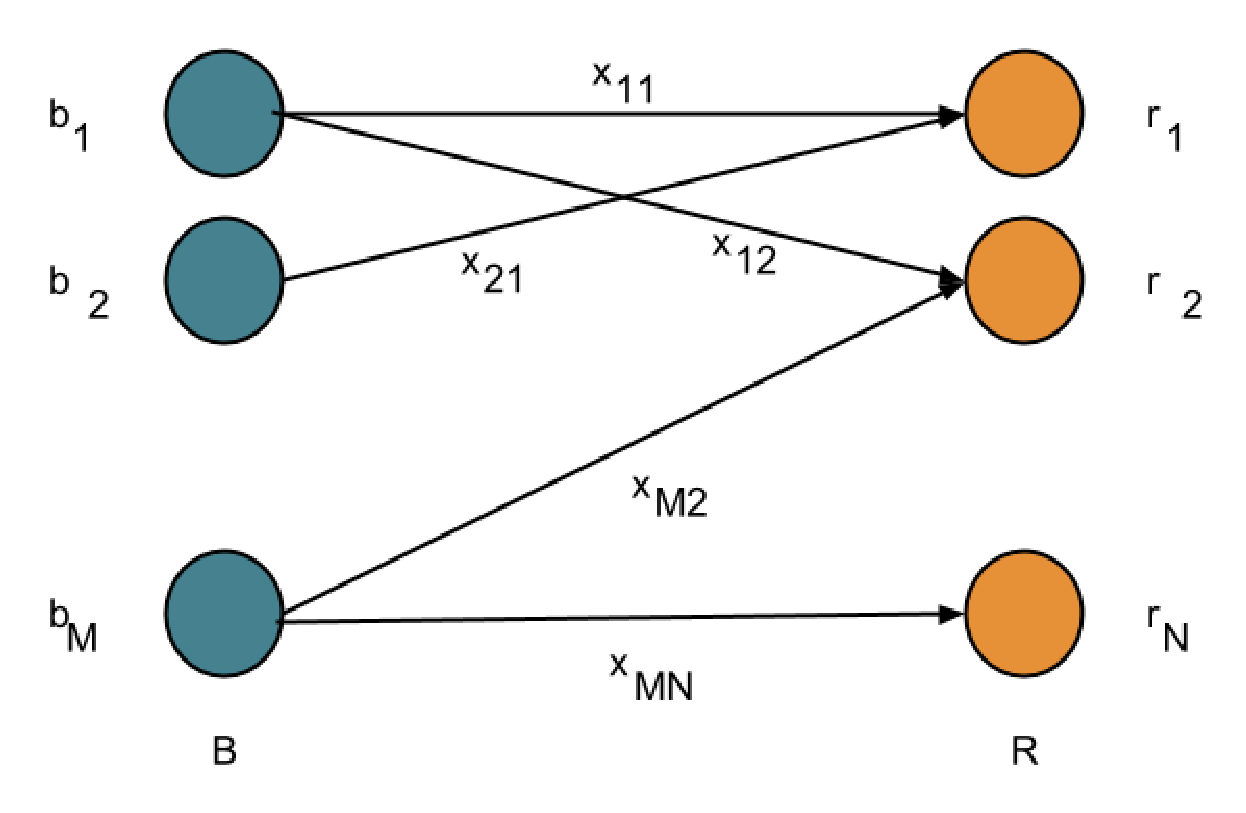
\includegraphics[height=5cm]{./images/rap.eps}
    \caption{A pictorial example of the Recipe Approximation Problem.}
  \end{figure}
\end{frame}

\begin{frame}[ctb!]
  \frametitle{Recipe Approximation Problem - Set Up} 

  An $\ell_1$ norm approximation formulation is used.\vspace{0.2cm}
  
  The objective function and constraints are comprised of properties of the
  determined solution.\vspace{0.2cm}

  The constraint properties are required to be met within some error, whereas
  the residual of the objective property is minimized.
\end{frame}

\begin{frame}[ctb!]
  \frametitle{Recipe Approximation Problem - Objective}

  In the current formulation, matching the target recipe is the objective.
  
  The residual is defined as
  \begin{equation}\label{eqs:residual}
    \vec{y_{t}} = \left| M \cdot \vec{x_{t}}  - m_t \vec{I_{t}} \right|.
  \end{equation}

  Given
  \begin{itemize}
    \item a barrel mass matrix $M$, i.e., $I_b * m_b$ for each barrel
    \item a feasible solution for a target recipe, $x_t$
  \end{itemize}

  The sum of residuals is minimized, using a weighting factor, $c_t$,
  \begin{equation}\label{rap-obj}
    \min_{z} \:\: z = \sum_{t \in T} \vec{c_{t}}^{\top} \cdot \vec{y_{t}}
  \end{equation}
\end{frame}

\begin{frame}[ctb!]
  \frametitle{Recipe Approximation Problem - Objective Weights}

  Issues with strictly matching recipes include:
  \begin{enumerate}
    \item presence of contaminants
    \item relative importance of fertile vs. fissile isotopes
  \end{enumerate}

  \vspace{0.2cm}

  A weighting factor is used to normalize contributions to the objective
  function:
  \begin{equation}\label{eqs:weights}
    c_{i,t} = 
    \begin{cases}
      \frac{1}{m_{i,t}} & \text{if } i \in I_{t} \\
      \frac{1}{m_{t}}   & \text{if } i \not\in I_{t}
    \end{cases}
  \end{equation}  
\end{frame}

\begin{frame}[ctb!]
  \frametitle{Recipe Approximation Problem - Mass Constraint}

  The mass differential is constrainted
  \begin{itemize}
    \item the solution should have approximately the same mass as the target
    \item a maximum violation, $\epsilon_{m}$, is provided
  \end{itemize}
  
  \begin{equation}\label{eqs:mass-constraint-simple}
    \epsilon_{m} \geq \left| m_{x_t} - m_{t} \right|.
  \end{equation}
\end{frame}

\begin{frame}[ctb!]
  \frametitle{Recipe Approximation Problem - Neutronics Constraint}

  A neutronics parameter is constrainted
  \begin{itemize}
    \item the solution should behave similar neutronically to the target
    \item neutron reproduction factor, $\eta$, is chosen
    \item $\eta$ is a function solely of the recipe, not reactor geometry, etc.
  \end{itemize}
\end{frame}

\begin{frame}[ctb!]
  \frametitle{Recipe Approximation Problem - Neutronics Constraint}

  $\eta$ is defined for a homogeneous material as:
  \begin{equation}
    \label{eqs:eta_micro}
    \eta_{t} = \frac{\sum_{i \in I_t} \nu^{i} \sigma_{f}^{i} N^{i}} {\sum_{i
        \in I_t} \sigma_{a}^{i} N^{i}},
  \end{equation}

  with physical constants:
  \begin{itemize}
    \item $\nu^{i}$ - the average number of neutrons produced by fission of isotope $i$
    \item $\sigma_{f}^{i}$ - the microscopic fission cross section for isotope $i$
    \item $\sigma_{a}^{i}$ - the microscopic absorption cross section for isotope $i$
    \item $N^i$ - the number density of isotope $i$
  \end{itemize}
\end{frame}

\begin{frame}[ctb!]
  \frametitle{Recipe Approximation Problem - Neutronics Constraint}

  From the perspective of mixing of barrels, one can define the reproduction
  factor of a proposed solution as:

  \begin{equation}
    \label{eqs:eta_simple}
    \eta_{x_t} = \frac{\sum_{b \in B} \eta_{b}^{+} x_{b, t}}
        {\sum_{b \in B} \eta_{b}^{-} x_{b, t}}
  \end{equation}

  Where $\eta_b^+$ and $\eta_b^-$ are defined as:

  \begin{equation}
    \label{eqs:eta_+}
    \eta_{b}^{+} \equiv \sum_{i \in I_{b}} \nu^{i} \sigma_{f}^{i} N_{b}^{i}
  \end{equation}

  \begin{equation}
    \label{eqs:eta_-}
    \eta_{b}^{-} \equiv \sum_{i \in I_{b}} \sigma_{a}^{i} N_{b}^{i}
  \end{equation}
  
\end{frame}

\begin{frame}[ctb!]
  \frametitle{Recipe Approximation Problem - Neutronics Constraint} 

  This separation allows one to write the neutronics constraint, given a maximum
  possible violation, $\epsilon_{\eta}$, as:

  \begin{equation}
    \label{eqs:eta_linear}
    \epsilon_{\eta} \sum_{b \in B} \eta_{b}^{-} x_{b,t} \geq
    \left| \sum_{b \in B} \eta_{b}^{+} x_{b,t}
    - \eta_{t} \sum_{b \in B} \eta_{b}^{-} x_{b,t} \right|
  \end{equation}  
\end{frame}

\begin{frame}[ctb!]
  \frametitle{Recipe Approximation Problem - Formulation}

  The full formulation for the RAP is then:
  \fontsize{7pt}{\baselineskip}\selectfont
  %%% 
  \begin{subequations}\label{eqs:rap}
    \begin{align}
      %%
      \min_{z} \:\: & 
      z = \sum_{t \in t} \vec{c_{t}}^{\top} \cdot \vec{y_{t}}
      & \label{eqs:rap_obj} \\
      %%
      \text{s.t.} \:\: &
      \vec{y_{t}} = \left| M \cdot \vec{x_{t}}  - m_t \vec{I_{t}} \right|
      &
      \forall t \in T \label{eqs:rap_iso} \\
      %%
      &
      \epsilon_{m} \geq \left| \sum_{b \in B} m_{b} x_{b, t} - m_{t} \right|
      & 
      \forall t \in T \label{eqs:rap_mass} \\
      %%
      &
      \epsilon_{\eta} \sum_{b \in B} \eta_{b}^{-} x_{b, t} \geq 
      \left| \sum_{b \in B} \eta_{b}^{+} x_{b, t} - 
      \eta_{t} \sum_{b \in B} \eta_{b}^{-} x_{b, t} \right|
      & 
      \forall t \in T \label{eqs:rap_eta} \\
      &
      \sum_{t \in T} x_{b, t} \leq 1
      & 
      \forall b \in B \label{eqs:rap_conserv} \\
      &
      x_{b, t} \in \left[ 0, 1 \right]
      & 
      \forall b \in B, \forall t \in T  \label{eqs:rap_x}
      %%
    \end{align}
  \end{subequations}
  %%% 
\end{frame}

\begin{frame}[ctb!]
  \frametitle{Recipe Approximation Problem - Research Questions} 

  Four primary research questions exist:

  \begin{enumerate}
    \item Does barrel size affect the accuracy of matches?
    \item Is isotopic ``closeness'' or neutronics parameter ``closeness'' the
      better objective function value?
    \item How to delineate between fast and thermal recipes?
    \item Are additional neutronics constraints helpful?
  \end{enumerate}
\end{frame}

\begin{frame}[ctb!]
  \frametitle{Next Steps} 
  
  \begin{itemize}
    \item all work will be done in the
      \href{github.com/cyclus/cyclus}{\Cyclus} code base, incorporating
      continuous integration and unit testing
    \item the \Cyclus team has identified the one and two-tier fuel cycles
      proposed in the recent Dynamic Systems Analysis Report for Nuclear Fuel
      Recycle (DSARR) \cite{dixon_dynamic_2008} as targets for
      development
    \item \Cyclus requires additional capability for modeling instances of
      multiple commodity supply/demand
    \item the proposed Information Gathering mechanism can supply this capability
      and provide downstream flexibility for future work
  \end{itemize}
\end{frame}

\begin{frame}[ctb!]
  \frametitle{Next Steps} 

  \begin{itemize}
    \item the LP formulation of the GFCTP will be implemented for this simple
      case
    \item the DSAR scenario will be extended to include multiple regions to
      provide a proof-of-principle example of preference-based material flow
    \item the MILP formulation for the GFCTP will then be implemented
    \item comparisons in run time and output will be observed, and, depending on
      outcomes, acceleration methods, such as cutting planes and preprocessing,
      will be investigated
    \item COIN-OR\cite{lougee_common_2003} open source libraries will be used
  \end{itemize}
\end{frame}

\begin{frame}[ctb!]
  \frametitle{Next Steps} 
  
  \begin{itemize}
    \item initially, a ``naive'' advanced fabrication facility will be used
    \item the RAP will be implemented 
    \item comparisons will be made with current approaches (e.g. COSI's equivalence method)
    \item simulation-level effects will be investigated (e.g., barrel size)
    \item again, COIN-OR open source libraries will be used
  \end{itemize}
\end{frame}
